\documentclass[french,12pt]{report}
\input{preambule_17-18}
\input{commandes_cecile_2019}
\input{perso_cecile_2019}

\begin{document}
\fancyhf{}


\newgeometry{includeheadfoot, top=1cm, bottom=0.8cm, right=1.5cm, left=1.5cm}



\chapter{Loi normale croquis}


espérance 1 écartype 2

\begin{center}
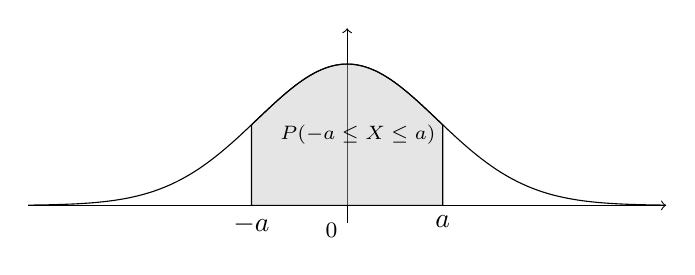
\begin{tikzpicture}[x=0.9cm,y=10.0cm,scale=0.9]
%\draw [color=gray, xstep=1.0cm,ystep=1.0cm] (-5,-0.025) grid (6,0.25);
\draw[->,color=black] (-4,0) -- (6,0);

\draw[->,color=black] (1,-0.025) -- (1,0.25);

\draw[color=black] (1,-10pt) node[left] {\footnotesize $0$};


\clip(-4.,-0.04) rectangle (6.,0.25);
\draw[color=black,fill=lightgray,fill opacity=0.4, smooth,samples=50,domain=-0.5:2.5] plot(\x,{e^((-(\x-1)^2)/4)/(2*sqrt(pi*2))}) -- (2.5,0) -- (-0.5,0) -- cycle;
\draw[smooth,samples=100,domain=-6.0:9.0] plot(\x,{e^((-((\x)-1)^2)/4)/(2*sqrt(pi*2))});
\draw(-0.5,0)node [below]{$-a$};
\draw(2.5,0)node[below]{$a$};
\draw(-0.2,0.1)node[right]{\scriptsize $P(-a\leq X\leq a)$};

\end{tikzpicture}
\end{center}

\begin{center}
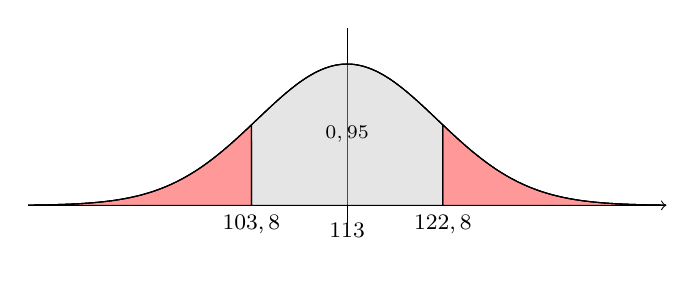
\begin{tikzpicture}[x=0.9cm,y=10.0cm,scale=0.9]

\draw[->,color=black] (-4,0) -- (6,0);

\draw[-,color=black] (1,-0.025) -- (1,0.25);

\draw[color=black] (1,-10pt) node[] {\footnotesize $113$};

\clip(-4.,-0.1) rectangle (6.,0.25);

\draw[color=black,fill=lightgray,fill opacity=0.4, smooth,samples=50,domain=-0.5:2.5] plot(\x,{e^((-(\x-1)^2)/4)/(2*sqrt(pi*2))}) -- (2.5,0) -- (-0.5,0) -- cycle;
\draw[smooth,samples=100,domain=-6.0:9.0] plot(\x,{e^((-((\x)-1)^2)/4)/(2*sqrt(pi*2))});

\draw[color=black,fill=red,fill opacity=0.4, smooth,samples=50,domain=-4:-0.5] plot(\x,{e^((-(\x-1)^2)/4)/(2*sqrt(pi*2))}) -- (-0.5,0) -- (-4,0) -- cycle;

\draw[color=black,fill=red,fill opacity=0.4, smooth,samples=50,domain=2.5:6] plot(\x,{e^((-(\x-1)^2)/4)/(2*sqrt(pi*2))}) -- (6,0) -- (2.5,0) -- cycle;
\draw[smooth,samples=100,domain=-6.0:9.0] plot(\x,{e^((-((\x)-1)^2)/4)/(2*sqrt(pi*2))});
\draw(-0.5,0)node [below]{\footnotesize $103,8$};
\draw(2.5,0)node[below]{\footnotesize $122,8$};
\draw(1,0.1)node[]{\scriptsize $0,95$};

\end{tikzpicture}
\end{center}


\end{document} 